\index{System! monoaminerg}

Die Signalübertragung zwischen zwei Neuronen beruht bei chemischen Synapsen auf der Freisetzung von Neurotransmittern in den synaptischen Spalt.
Die Transmitter werden in Gruppen eingeteilt, jeweils nach ihrer chemischer Strukturformel. Es wird zwischen drei Hauptklassen unterschieden: den Aminosäuren, Aminen und Peptiden. \textsuperscript{\cite[Kap.~6]{neurowissenschaften_baer}}

In diesem Kapitel werden wir uns mit den Monoaminen beschäftigen.
Der Begriff 'Monoamine' \index{Monoamin} beschreibt biochemische Stoffe, die einen aromatischen Ring aufweisen. Sie werden ausgehend von Aminosäuren synthetisiert. Zu den Monoaminen gehören Serotonin und Histamin, sowie die Catecholamine Adrenalin, Noradrenalin und Dopamin.
Die Catecholamine werden ausgehend von der Aminosäure Tyrosin synthetisiert. Ein wichtiger Bestandteil des Synthesewegs (fig.~\ref{fig:synthese_catecholamine}) ist die Tyrosin-Hydroxylase \textsuperscript{\cite[Kap.~13]{kandel2013principles}}, die bei der immunhistochemischen Färbung der Schnitte als Nachweis der Catecholamine Dopamin und Noradrenalin diente. In catecholaminergen Kerngebieten können sowohl die Somata als auch die zugehörigen Fasern angefärbt werden. In Kerngebieten, die lediglich Projektionen aus den catecholaminergen Geweben erhalten, werden ausschließlich die eintreffenden Fasern eingefärbt.
Jeder catecholaminerge Neurotransmitter bildet sein eigenes System, zu dem die Synthese des Transmitters, die Signalkaskade am synaptischen Spalt und die postsynaptische Wirkung gezählt wird. Die serotonergen und noradrenergen Nuclei des Gehirns sind im caudalen Hirnstamm, in der Formatio reticularis, konzentriert \textsuperscript{\cite[Kap.~7]{trepel2011neuroanatomie}}.
Der Großteil des Dopamins wird in rostraleren Kerngebieten synthetisiert \textsuperscript{\cite[Kap.~63]{kandel2013principles}}.
Die monoaminergen Neurone besitzen weitreichende Projektionen innerhalb des zentralen Nervensystems, die sowohl in sensorische und motorische, als auch in autonome und kognitive Funktionen involviert sind \textsuperscript{\cite[Kap.~9]{crossman2014neuroanatomy}}.

\begin{figure}[H]
    \centering
    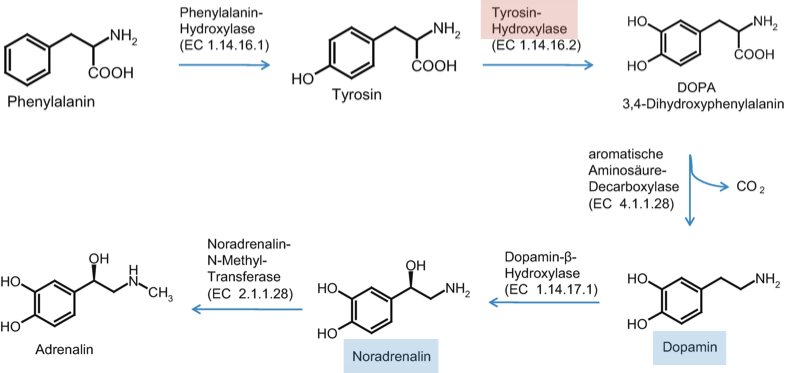
\includegraphics[width=\textwidth]{pictures/Bilder_monoamine_systeme/Synethese_Katecholamine.png}
    \caption[Synthese Catecholamine]{\textbf{Synthese Catecholamine.} Die Catecholamine, zu denen sowohl Dopamin als auch Noradrenalin (blau) gehören, werden ausgehend von der Aminosäure Tyrosin synthetisiert. Wichtiger Bestandteil des Synthesewegs ist die Tyrosin-Hydroxylase (rot), die bei der immunhistochemischen Färbung der Schnitte als Nachweis der Catecholamine diente.
    Abbildung aus \textit{Lexikon der Medizinischen Laboratoriumsdiagnostik}, Hubl \textsuperscript{\cite{Hubl2019}}}
    \label{fig:synthese_catecholamine}
\end{figure}{}
